\documentclass[xcolor=table]{beamer}

\usepackage[french]{babel}
\usepackage[latin1]{inputenc}
\usepackage[normalem]{ulem}
\usepackage[T1]{fontenc}
\usepackage{fancyhdr}   %% Pour la gestion des num�ros de page
\usepackage{graphicx}
\usepackage{amsmath}
\usepackage{mathrsfs}
\usepackage{amsfonts}
\usepackage{palatino}        %% Palatino fonts
\usepackage{mathptm}        %% PostScript Type 1 math fonts
\usepackage{dsfont} %% Pour mathds
\usepackage{color}
%%\usepackage{pstricks}
\usepackage{xmpmulti}
\usepackage{hyperref}
\usepackage{multimedia}
\usepackage{multirow}
%\usepackage[table]{xcolor}
\usepackage{fourier-orns}
\usepackage{subfigure}
\usepackage{tikz}

\DeclareMathAlphabet{\mathpzc}{OT1}{pzc}{m}{it}

\definecolor{vert}{rgb}{0.07,0.7,0.00}
\definecolor{gris}{gray}{0.70}
\definecolor{gris2}{gray}{0.95}
\definecolor{bleu}{rgb}{0.19,0.19,0.68}

%table setting
\newcommand\T{\rule{0pt}{2.6ex}}
\newcommand\B{\rule[-1.2ex]{0pt}{0pt}}
\renewcommand{\thesubfigure}{\thefigure.\arabic{subfigure}}

\usetheme{allee_marine} %voir fichier beaerthemeallee_marine.sty   ==> \usetheme{allee_marine}


%%%%%%%%%%%%%%%%%%%%%%%%%% Pr�sentation du document %%%%%%%%%%%%%%%%%%%%%%%%%%
\title[Master 1 Project]{User requirements}
\author[Etienne CAILLAUD, Thomas LE BRIS, Ibrahima GUEYE, Ga�tan ADIER]{\textbf{Etienne CAILLAUD, Thomas LE BRIS, Ibrahima GUEYE, Ga�tan ADIER}}
\institute [XLIM-SIC UMR CNRS 7252]{\textbf{XLIM-SIC Laboratory UMR CNRS 7252, Poitiers, France}}
\date{}

%%%%%%%%%%%%%%%%%%%%%%% Num�ro de pages en bas � gauche %%%%%%%%%%%%%%%%%%%%%%
\addtobeamertemplate{footline}{\color{blue}\hfill\insertframenumber/\inserttotalframenumber}

\pgfdeclareimage[height=96mm,width=128mm]{nombidon}{mood_eye_light}
\setbeamertemplate{background}{\pgfuseimage{nombidon}}

\pgfdeclareimage[height=96mm,width=128mm]{nombidon2}{mood_eye_light}
\setbeamertemplate{background}{\pgfuseimage{nombidon2}}

%%----------------------------------------------------------------------------
%% A chaque d�but de sous-section : g�n�re une table des mati�res
%%----------------------------------------------------------------------------
\AtBeginSection[]
{
   \setbeamertemplate{background}{\pgfuseimage{nombidon}}
   \begin{frame}<beamer>
    \frametitle{Outline}
    \tableofcontents[currentsection, hideallsubsections] %% affiche la section courante et les autres en gris�, masque les sous-sections
   \end{frame}
  \setbeamertemplate{background}{\pgfuseimage{nombidon2}}
}

\AtBeginSubsection[]
{
  \setbeamertemplate{background}{\pgfuseimage{nombidon}}
  \begin{frame}<beamer>
    \tableofcontents[sectionstyle=show/shaded,subsectionstyle=show/shaded/hide, subsubsectionstyle =hide]
  \end{frame}
   \setbeamertemplate{background}{\pgfuseimage{nombidon2}}
}

\AtBeginSubsubsection[]
{
  \setbeamertemplate{background}{\pgfuseimage{nombidon}}
  \begin{frame}<beamer>
    \tableofcontents[sectionstyle=show/shaded,subsectionstyle=show/shaded/hide,subsubsectionstyle =show/shaded/hide]
  \end{frame}
   \setbeamertemplate{background}{\pgfuseimage{nombidon2}}
}


%%%%%%%%%%%%%%%%%%%%%%%%%%%%%%%%%%%%%%%%%%%%%%%%%%%%%%%%%%%%%%%%%%%%%%%%%%%%%%
%%%%%%%%%%%%%%%%%%%%%%%%%%%%                       %%%%%%%%%%%%%%%%%%%%%%%%%%%
%%%%%%%%%%%%%%%%%%%%%%%%%%     D�BUT DU DOCUMENT     %%%%%%%%%%%%%%%%%%%%%%%%%
%%%%%%%%%%%%%%%%%%%%%%%%%%%%                       %%%%%%%%%%%%%%%%%%%%%%%%%%%
%%%%%%%%%%%%%%%%%%%%%%%%%%%%%%%%%%%%%%%%%%%%%%%%%%%%%%%%%%%%%%%%%%%%%%%%%%%%%%
\begin{document}
\graphicspath{{images/}}
\setbeamercolor{block title example}{bg = gray}

\begin{frame}
    \vspace{-1.5cm}
    \begin{tikzpicture}[remember picture,overlay]
        \node[xshift=0cm, above=8.6cm] at (current page.south west)
        {
\includegraphics[width=40cm,height=0.9cm]{cache_titre.png}};
        \node[xshift=2cm, above=2.8cm] at (current page.south west)
        {
\includegraphics[height=1.5cm]{Xlim.png}};
        \node[xshift=11cm, above=3cm] at (current page.south west)
        {
\includegraphics[height=1cm]{logo_une.jpg}};
        \node[xshift=6.5cm, above=0.7cm] at (current page.south west)
        {
\includegraphics[height=1.6cm]{Lifeclef.png}};
    \end{tikzpicture}
    \titlepage
\end{frame}

%%%%%%%%%%%%%%%%%%%%%%%%%%%%%%%%%%%%%%%%%%%%%%%%%%%%%%%%%%%%%%%%%%%%%%%%%%%%%%%%%%%%%%%%%%%%%%%%%%%%%
%%%%%%%%%%%                        D�but de la pr�sentation                       			 %%%%%%%%
%%%%%%%%%%%%%%%%%%%%%%%%%%%%%%%%%%%%%%%%%%%%%%%%%%%%%%%%%%%%%%%%%%%%%%%%%%%%%%%%%%%%%%%%%%%%%%%%%%%%%
\section{Project background}
%%-----------------------------------------------------------------------------------------
\begin{frame} \frametitle{Context and environment}
  \vspace{0.2cm}
    \begin{itemize}
     \item XLIM-SIC laboratory of Poitiers University.
     \vspace{0.3cm}
     \item Researching for new feature matching and indexing solutions for image retrieval and analysis.
     \vspace{0.3cm}
     \item Life CLEF contest 2015.
        \begin{itemize}
          \item CLEF $=$ Cross Language Evaluation Forum
          \item International contest for image retrieval
        \end{itemize}
    \end{itemize}
\end{frame}

%%-----------------------------------------------------------------------------------------
\begin{frame} \frametitle{Project goal}
%%-----------------------------------------------------------------------------------------
   \begin{itemize}
      \item Develop a software program for image retrieval.
        \begin{itemize}
          \item Embedding a new color texture feature
        \end{itemize}
      \vspace{0.3cm}
      \item Compare the obtained performances (CLEF challenge).
      \vspace{0.3cm}
      \item Relevant in our skill developments inside the training
        \begin{itemize}
          \item Image processing, computer sciences, classification and statistics
        \end{itemize}
      \vspace{0.3cm}
      \item Many educational topics related to this project.
        \begin{itemize}
          \item Project management, time constraints, deliverables, \ldots
        \end{itemize}
   \end{itemize}
\end{frame}
%%-----------------------------------------------------------------------------------------
\begin{frame} \frametitle{Scope of work}
%%-----------------------------------------------------------------------------------------
   \begin{itemize}
      \item Design a software program for image retrieval in database.
      \vspace{0.3cm}
      \item Adapt the last up to date designed color texture attributes (vectorial construction).
      \vspace{0.3cm}
      \item Compare last research results in color texture analysis in front of the Big-Data challenge.
   \end{itemize}
\end{frame}
%%-----------------------------------------------------------------------------------------
\begin{frame} \frametitle{Stakeholders}
%%-----------------------------------------------------------------------------------------
   \begin{itemize}
        \item Customer:
            Thierry Urruty.
        \vspace{0.3cm}
        \item People involved in the project:
            Thomas Le Bris, Ga�tan Adier, Ibrahima Gueye, Etienne Caillaud, David Helbert, No�l Richard.
        \vspace{0.3cm}
        \item End users:
            Economical structures in charge of large image database (Flicker, Google, CIBDI Angouleme, E�nden...).
      \end{itemize}
\end{frame}
%%-----------------------------------------------------------------------------------------
\begin{frame} \frametitle{State of the art}
%%-----------------------------------------------------------------------------------------
\begin{overprint}
    \onslide<1>
    \begin{itemize}
      \item CLEF  $\rightarrow$ international competition between
        \begin{itemize}
          \item University laboratories
          \item Societies : IBM
        \end{itemize}
      \vspace{0.3cm}
      \item Automatic extraction of key-points (KP)
        \begin{itemize}
          \item Salient key-point
          \item Dense grid
        \end{itemize}
      \vspace{0.3cm}
      \item Texture or local information $\forall$ KP
        \begin{itemize}
          \item SIFT or/and SURF are the most used
          \item $C_2O$ being to compare
        \end{itemize}
    \end{itemize}

    %----------------------------------------------------------------
    \onslide<2>
    \begin{itemize}
      \item chosen approach as reference
        \begin{itemize}
          \item FINKI : top ten of lifeCLEF 2014.
          \item Multiscale triangular shape or opponent SIFT
        \end{itemize}
      \vspace{0.3cm}
      \item Challenge metrics from CLEF
        \begin{itemize}
          \item Mean of the average classification rate.
        \end{itemize}
    \end{itemize}

\end{overprint}
\end{frame}
%%-----------------------------------------------------------------------------------------

\section{Constraints}
\begin{frame} \frametitle{Deadlines}
%%-----------------------------------------------------------------------------------------
  \begin{figure}[ht]
    \centering
    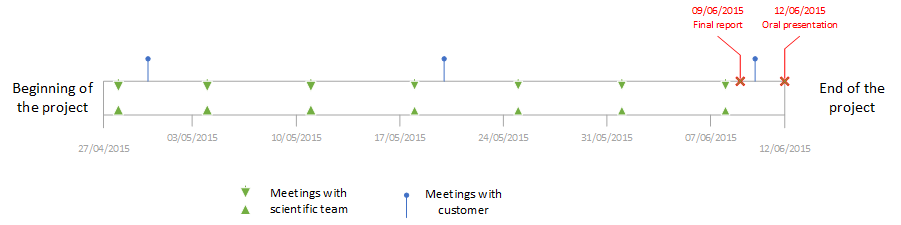
\includegraphics[scale=0.5]{TimelinePresentation.png}
    \caption{Gantt chart}
    \label{fig:image1}
  \end{figure}

   \begin{itemize}
      \item SCRUM meetings every morning.
   \end{itemize}

\end{frame}
%%-----------------------------------------------------------------------------------------

\section{Description of the final product}
\begin{frame} \frametitle{Software}
%%-----------------------------------------------------------------------------------------
   \begin{itemize}
      \item Software program able to calculate texture features for one image (argument of the executable file).
        \begin{itemize}
          \item Texture feature computation
          \item Image retrieval process using the CLEF databases
          \item Performance metrics from CLEF
        \end{itemize}
      \vspace{0.3cm}
      \item For each image
      \vspace{0.3cm}
      \begin{itemize}
            \item Create one directory for each image.
            \item One text file with all the information about the image
                \begin{itemize}
                  \item From the CLEF database.
                \end{itemize}
            \item One text file per descriptor/feature. One information per line
      \end{itemize}
   \end{itemize}
\end{frame}
%%-----------------------------------------------------------------------------------------
\begin{frame} \frametitle{Performance comparison}
%%-----------------------------------------------------------------------------------------
   \begin{itemize}
      \item Compare our results with the other laboratories.
        \begin{itemize}
          \item From the previous CLEF challenge
          \item Using CLEF challenge metrics
        \end{itemize}
      \vspace{0.3cm}
      \item Produce an analysis of the obtained performances
        \begin{itemize}
          \item Using the classical color texture features
          \item Using the new color texture feature proposed by XLIM-SIC
        \end{itemize}
      \vspace{0.3cm}
      \item Produce a technical report allowing to continue this project and the CLEF contest
   \end{itemize}
\end{frame}
%%-----------------------------------------------------------------------------------------

\section{Organization and project management}
%%-----------------------------------------------------------------------------------------
\begin{frame} \frametitle{Schedule}
%%-----------------------------------------------------------------------------------------
  \begin{figure}[ht]
    \centering
    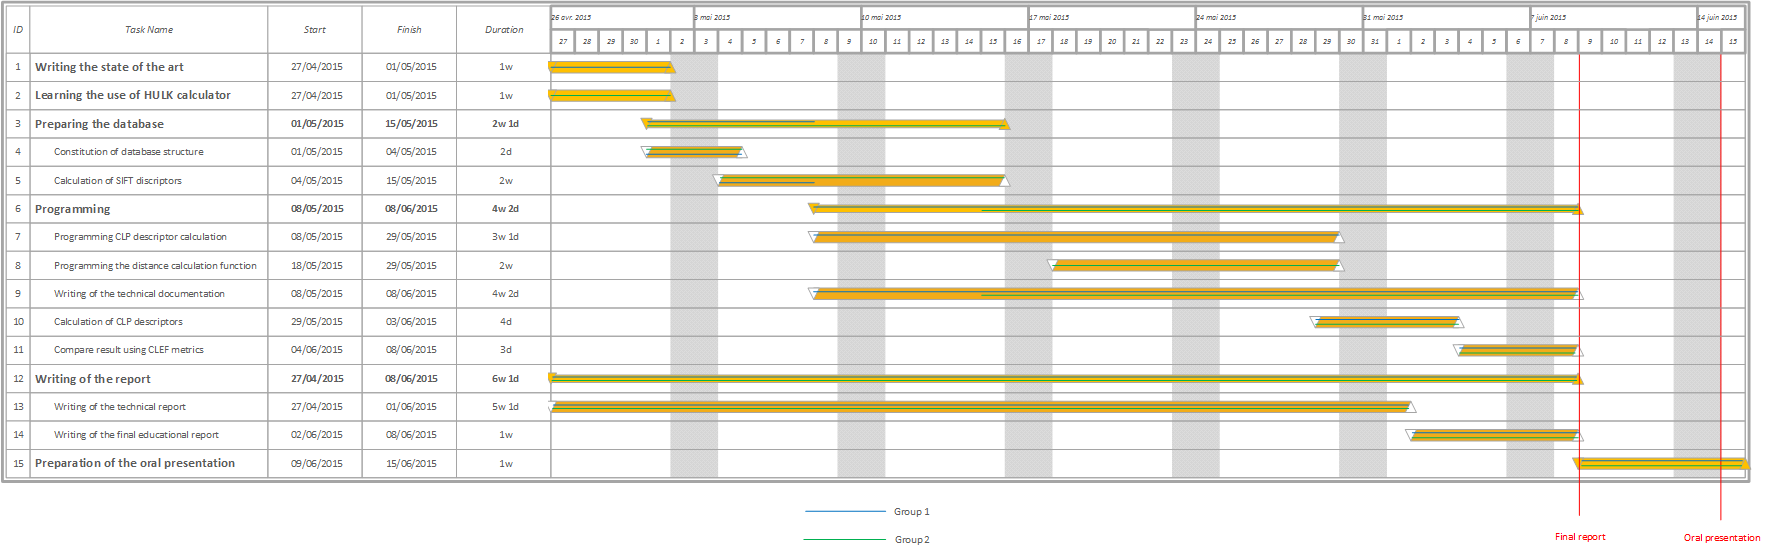
\includegraphics[scale=0.25]{Diagramme_de_Gantt.png}
    \caption{Gantt chart}
    \label{fig:image1}
  \end{figure}
\end{frame}
%%-----------------------------------------------------------------------------------------
\begin{frame} \frametitle{Location}
%%-----------------------------------------------------------------------------------------
   \begin{itemize}
      \item Project classrooms (ON03/01/17) in SP2MI building.
   \end{itemize}
\end{frame}
%%-----------------------------------------------------------------------------------------

\section{Necessary resources for development}
\begin{frame} \frametitle{Resources}
%%-----------------------------------------------------------------------------------------

      \begin{itemize}
	   \item Connection to computing university server.
        \vspace{0.3cm}
	   \item Computers with Python edition tools.
        \vspace{0.3cm}
       \item Electrical outlets and internet access.
      \end{itemize}

\end{frame}
%%-----------------------------------------------------------------------------------------

\section{Conclusion}
\begin{frame} \frametitle{Conclusion}
%%-----------------------------------------------------------------------------------------
    \begin{itemize}
	   \item Using programming and image processing on new subject.
        \vspace{0.3cm}
	   \item Experience in project management.
        \vspace{0.3cm}
       \item Opportunity to participate in a contest.
      \end{itemize}
\end{frame}
%%-----------------------------------------------------------------------------------------


\section{}
\begin{frame} \frametitle{}
%%-----------------------------------------------------------------------------------------
    \begin{center}
        Thanks for attention
    \end{center}
\end{frame}
%%-----------------------------------------------------------------------------------------



\end{document}

